\documentclass[tikz,border=4pt]{standalone}
\usepackage{ctex}
\usepackage{amsmath}
\usepackage{pgfplots}
\pgfplotsset{compat=1.18}
\begin{document}
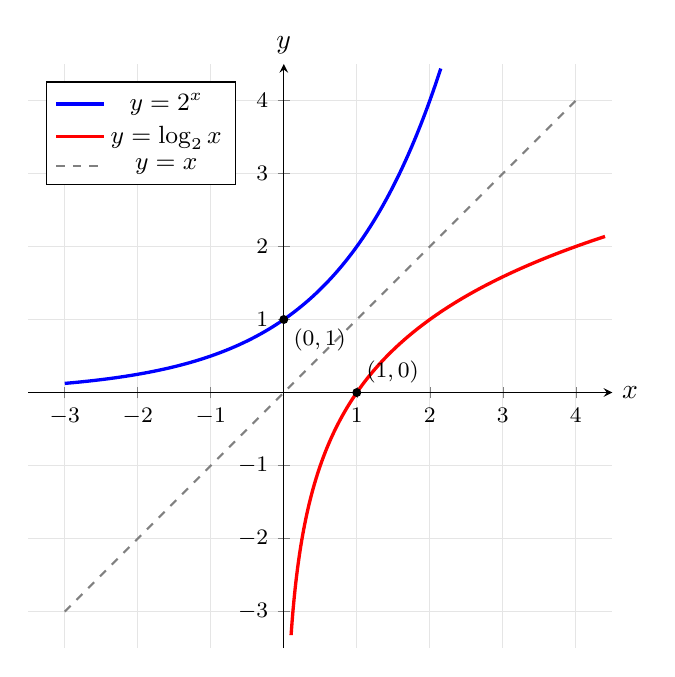
\begin{tikzpicture}
\begin{axis}[
    axis lines=middle,
    xmin=-3.5, xmax=4.5,
    ymin=-3.5, ymax=4.5,
    width=9cm, height=9cm,
    xlabel={$x$}, ylabel={$y$},
    xlabel style={right}, ylabel style={above},
    samples=300,
    grid=both,
    grid style={gray!20},
    legend pos=north west,
    legend style={font=\small},
    axis equal image,
    tick label style={font=\footnotesize},
]
\addplot[blue, very thick, domain=-3:2.15] {2^x};
\addlegendentry{$y=2^x$}
\addplot[red, very thick, domain=0.10:4.4] {ln(x)/ln(2)};
\addlegendentry{$y=\log_2 x$}
\addplot[gray, dashed, thick, domain=-3:4] {x};
\addlegendentry{$y=x$}
\addplot[only marks, mark=*, mark size=1.4pt, black] coordinates {(0,1) (1,0)};
\node[below right, font=\footnotesize] at (axis cs:0,1) {$(0,1)$};
\node[above right, font=\footnotesize] at (axis cs:1,0) {$(1,0)$};
\end{axis}
\end{tikzpicture}
\end{document}
